\documentclass[11pt, a4paper]{beamer}

% Packages
\usepackage[french]{babel}
\usepackage[utf8]{inputenc}
\usepackage[T1]{fontenc}
\usepackage{lmodern}
\usepackage{amsmath, amsthm}
\usepackage{amsfonts,amssymb}
% \usepackage[left=3.25cm, right=3.25cm, top=2.2cm, bottom=2.2cm]{geometry}

\usepackage{graphicx}
\usepackage{epsfig}
\usepackage{caption}
\usepackage{alltt}
% \usepackage[svgnames]{xcolor}
\usepackage{soul}
\usepackage{dsfont}
\usepackage{pstricks,pst-plot,pst-text,pst-tree,pst-eps,pst-fill,pst-node,pst-math}
\usepackage{listings}
\usepackage{eurosym}
\usepackage{extarrows}
%\usepackage{pdfpages}
\usepackage{helvet}
% Théorèmes
\usepackage{amsthm}
% \theoremstyle{definition} %par exemple, mais ce n'est pas utile pour la numérotation
% \newtheorem{theo}{Théorème}[chapter]
% \newtheorem{defi}[theo]{Définition}
% \newtheorem{prop}[theo]{Proposition}

\usecolortheme{seahorse}


% Commands
\newcommand{\w}{\widehat}
\newcommand{\F}{\mathcal{F}}
\renewcommand{\P}{\mbox{\textbf{P}}}
\newcommand{\E}{\mbox{\textbf{E}}}
\newcommand{\1}{\mbox{\textbf{1}}}
\renewcommand{\d}{\mbox{d}}

% Title
\title{Modélisation du système manguier--cécidomyies}
\author{}
\date{}

\begin{document}
 
 \begin{frame}
  \titlepage
 \end{frame}
 

\begin{frame}
\frametitle{Problématique}
Forts asynchronismes inter-- et intra-- arbres

\hspace*{1cm}$\longrightarrow$ Favorable au développement des ravageurs

\vspace*{1.5cm}

Leviers de gestion :
\begin{enumerate}
 \item Taille des manguiers
 \begin{itemize}
  \item Réduction des asynchronismes
 \end{itemize}
 \item Paillage du sol
 \begin{itemize}
  \item Réduction de l'émergence des cécidomyies des fleurs
 \end{itemize}
\end{enumerate}


\end{frame}



%% CE QUI A DÉJÀ ÉTÉ FAIT%

\begin{frame}
 \frametitle{Données}
 Plusieurs types de données : 
 \begin{enumerate}
  \item Dynamique des cécidomyies des fleurs
  \item Floraison
  \item Dégâts sur les inflorescences
  \item Températures
 \end{enumerate}
 \includegraphics[scale=0.38]{sol.png}
\end{frame}

%\begin{frame}
%\begin{figure}
%\centering
% 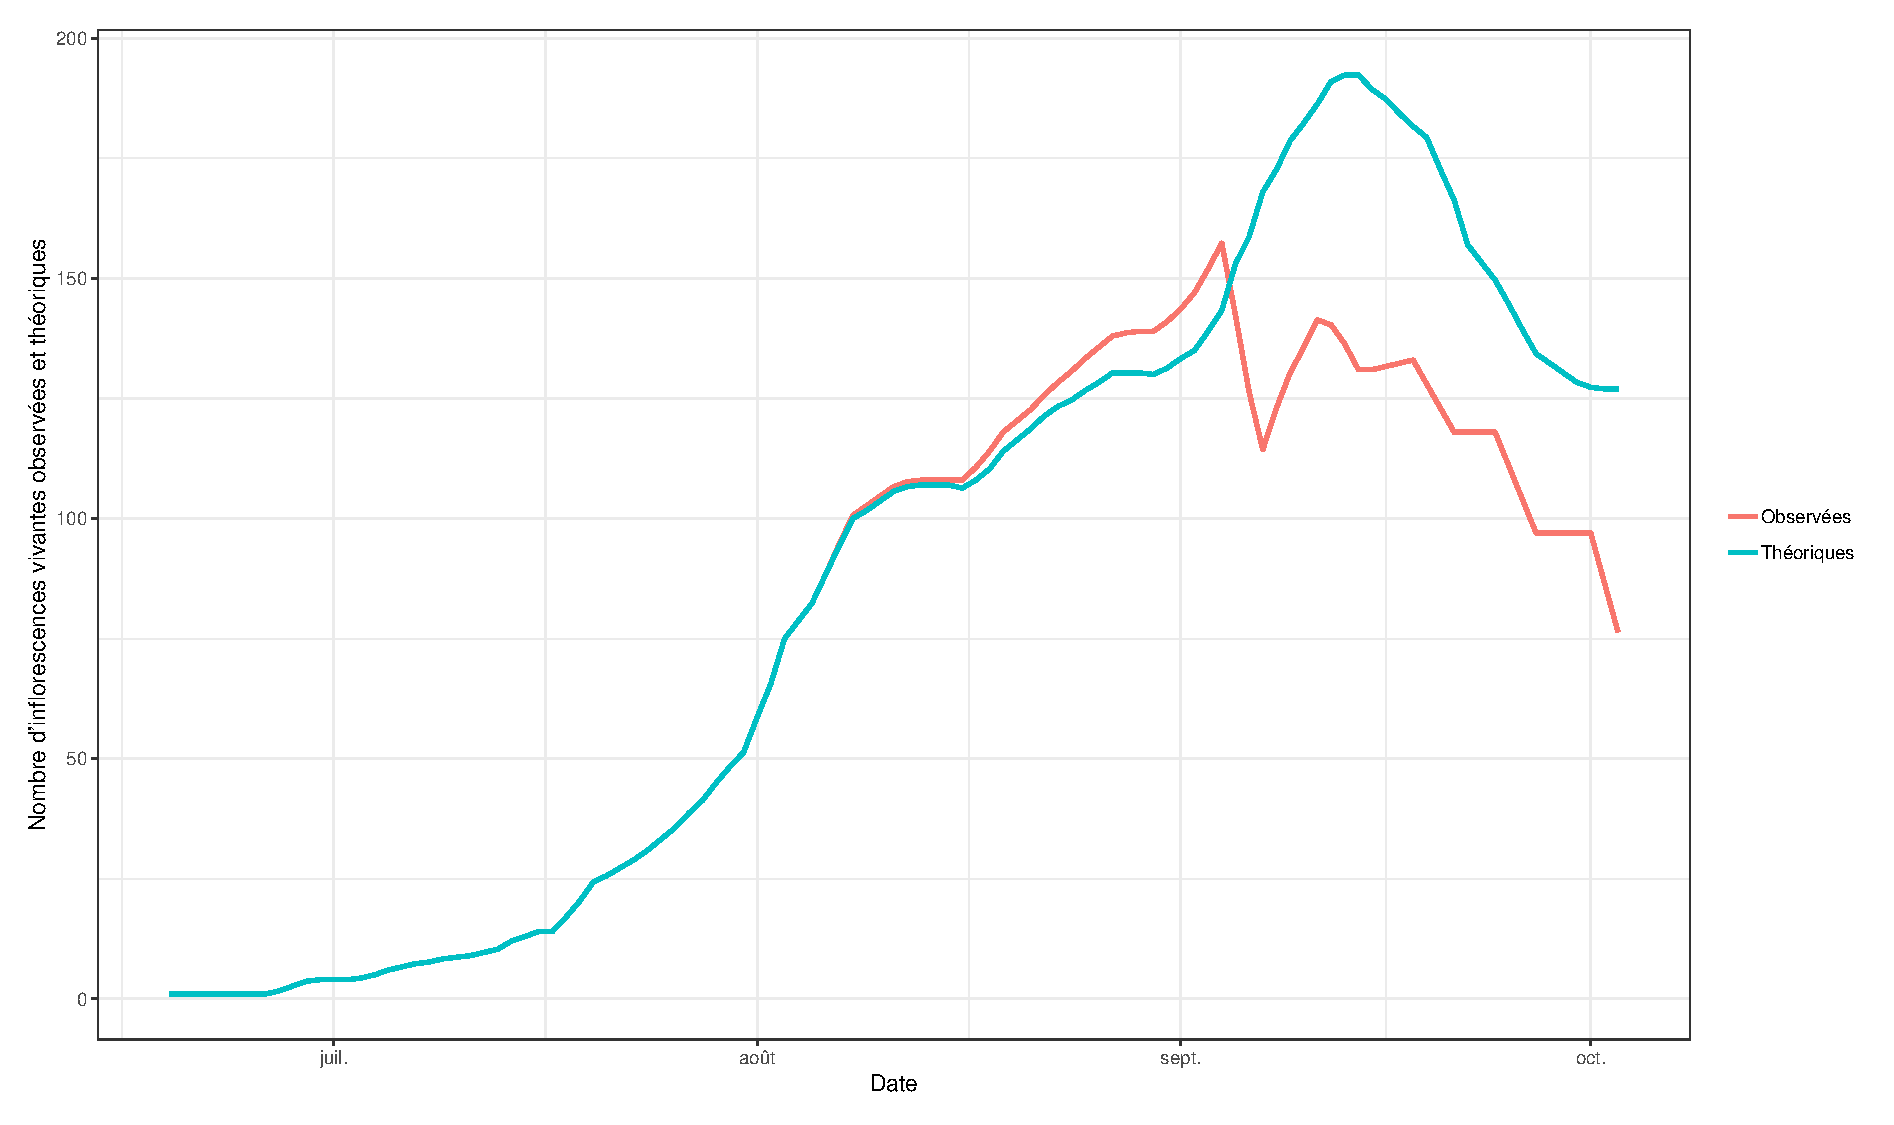
\epsfig{file=comp_obs_theo.eps, width = 10.8cm}
% \caption{Comparaison du nombre d'inflorescences vivantes obervées et théoriques (lissées avec une moyenne mobile d'ordre 3)}
%\end{figure}
%\end{frame}


\begin{frame}
 \begin{figure}
 \centering
 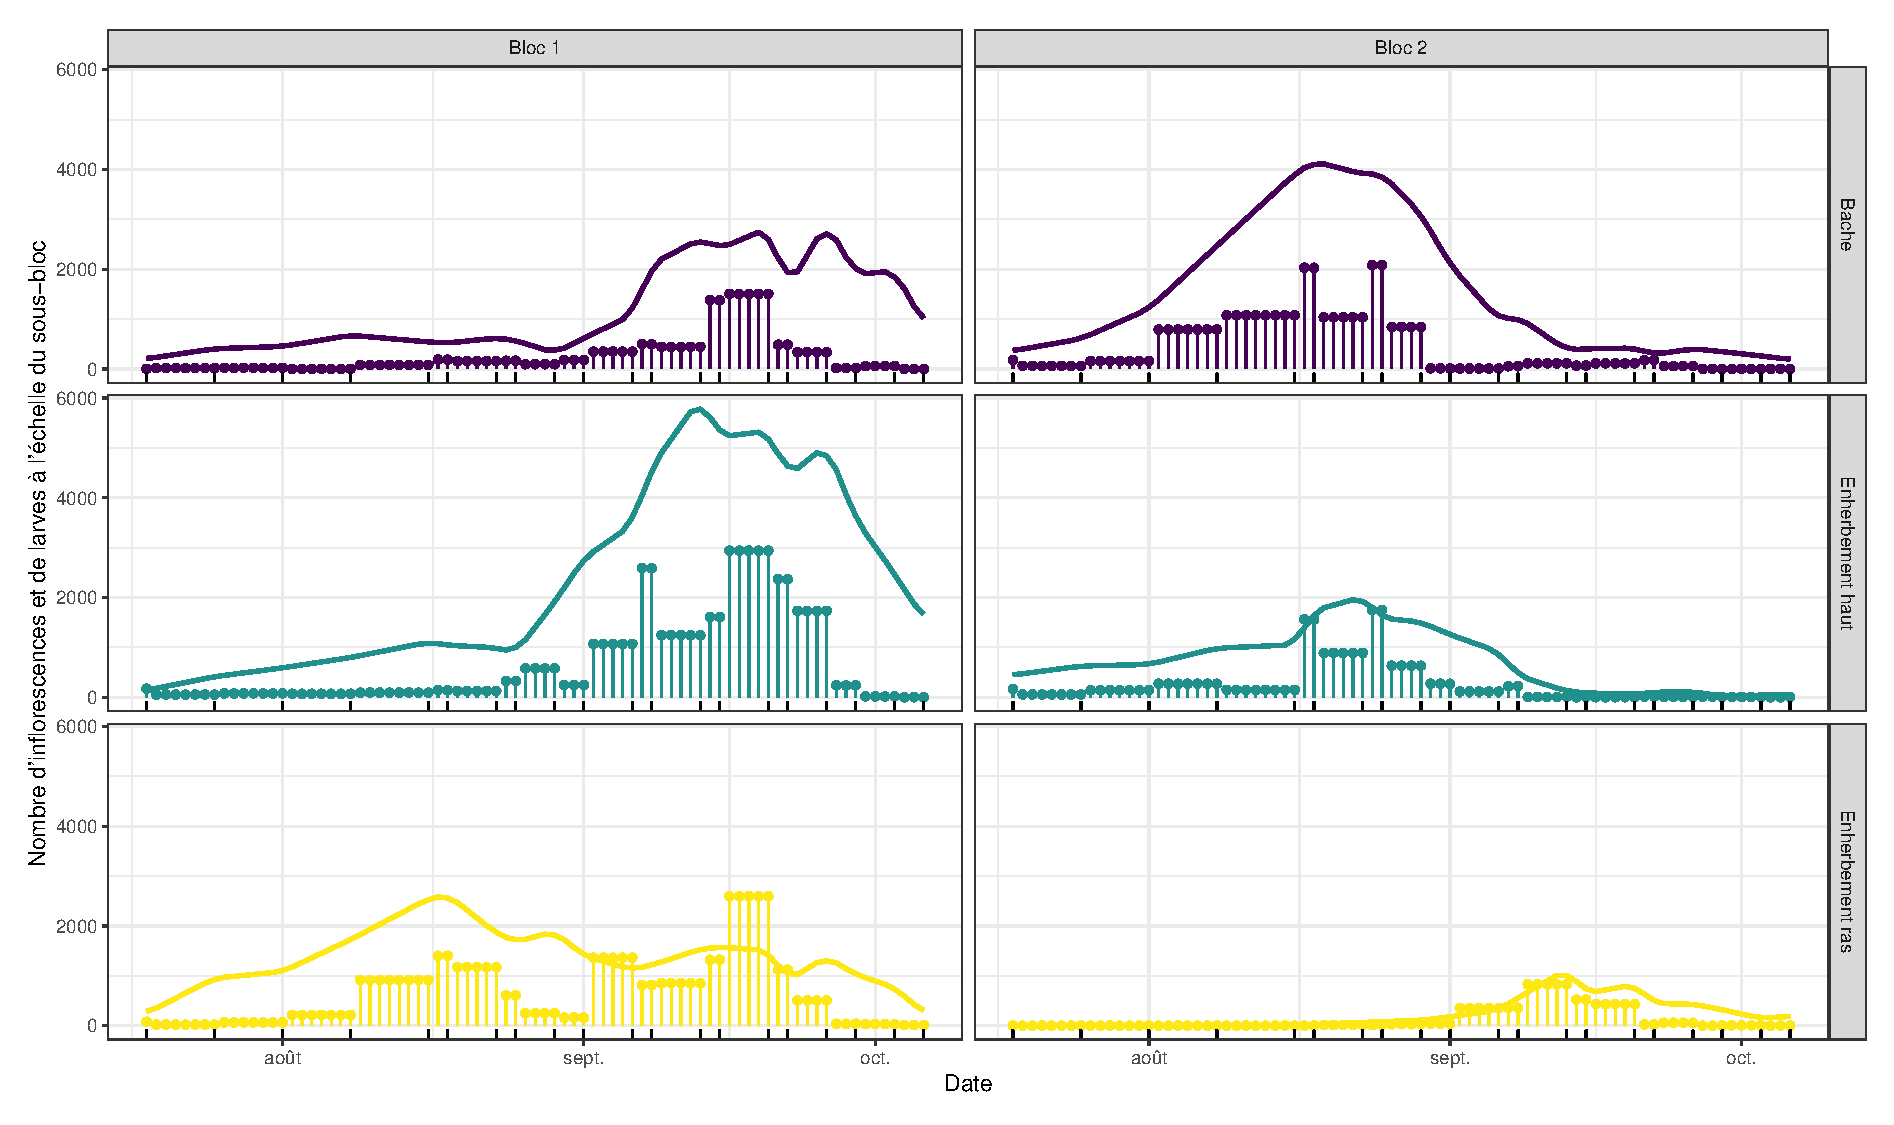
\epsfig{file=comparaison.eps, width = 10.8cm}
 % larves_grid_nolegend.pdf: 655x392 px, 72dpi, 23.11x13.83 cm, bb=0 0 655 392
 \caption{Comparaison du nombre de larves piégées (rapporté au jour) et du nombre d'inflorescences vivantes (lissé avec une moyenne mobile d'ordre 3). Les marqueurs noirs sur l'axe des abscisses représentent les dates de relevés des observations.}
\end{figure}
\end{frame}


\begin{frame}
 \begin{figure}
   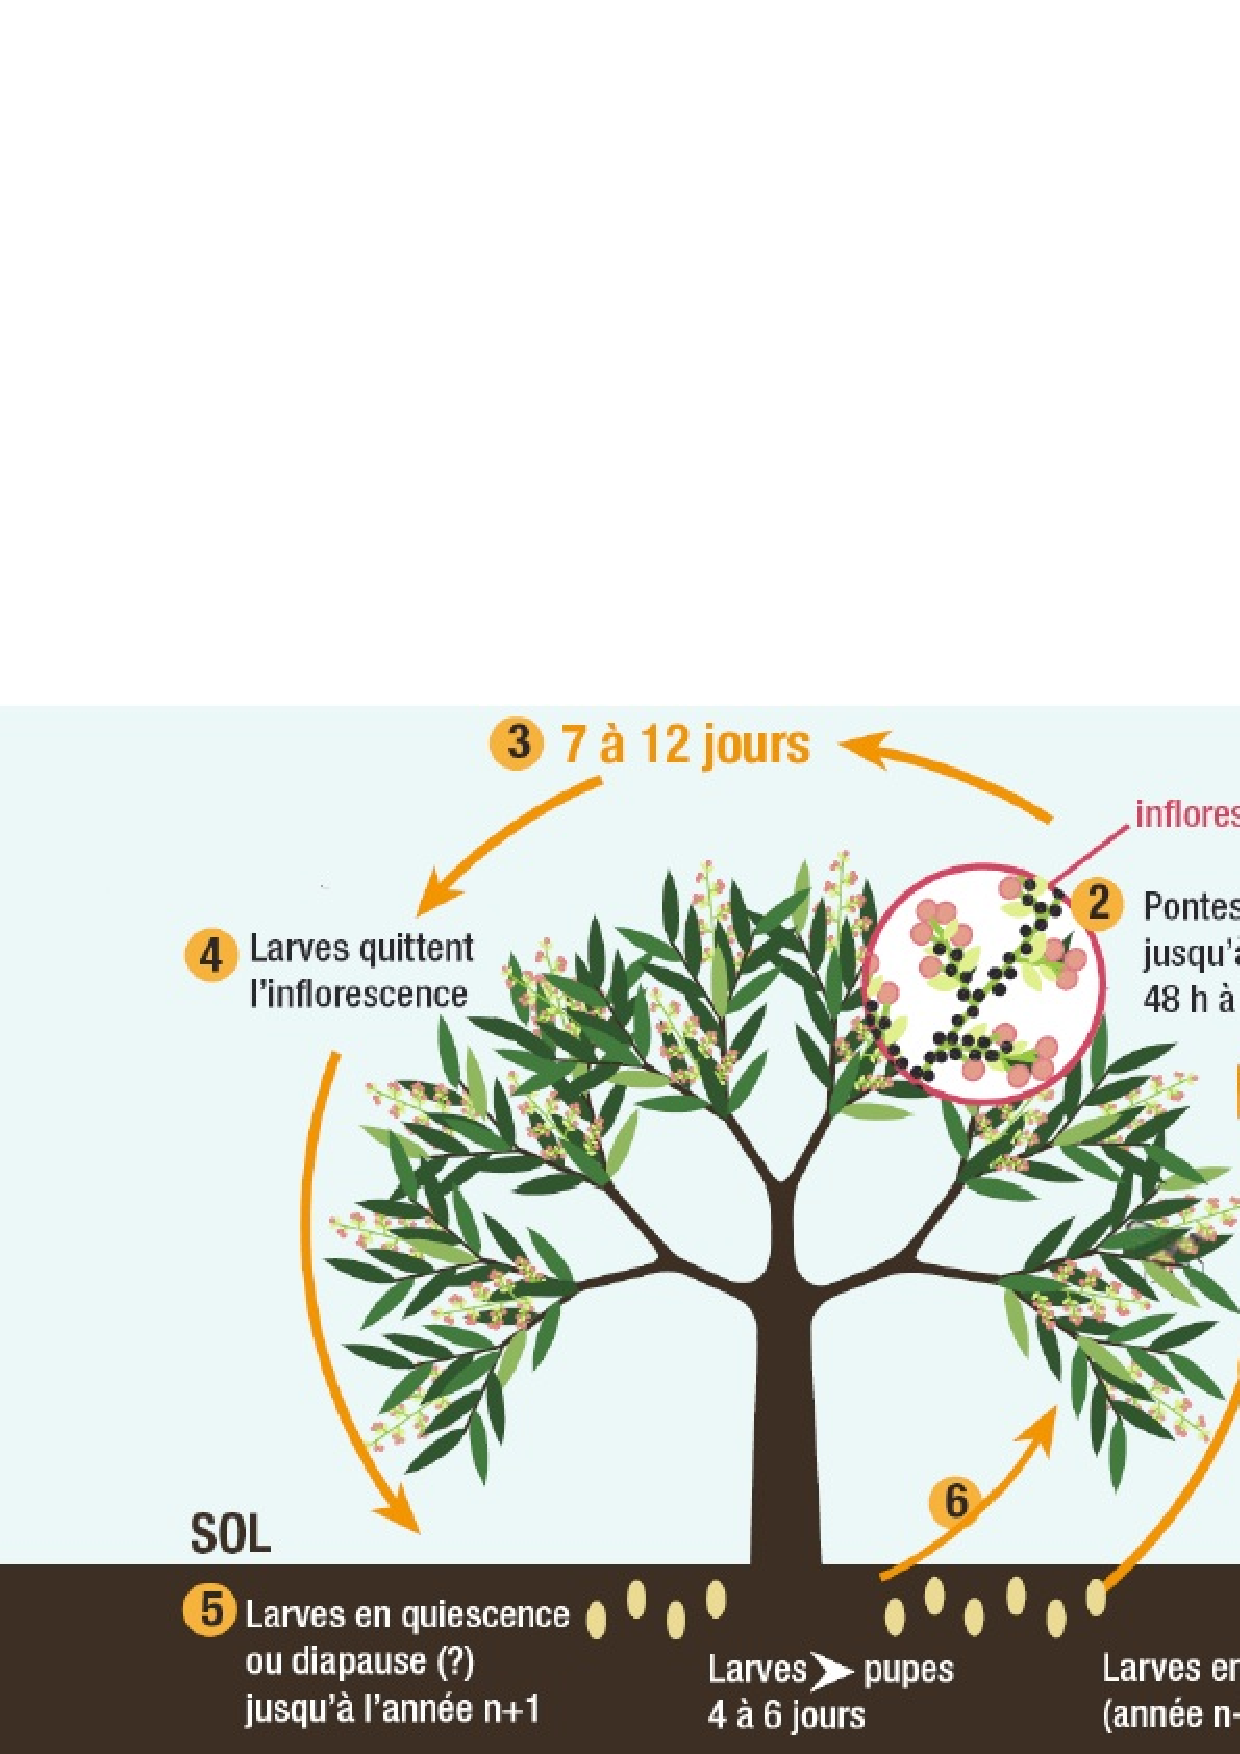
\includegraphics[scale=0.4]{cycle.png}
\caption{Cycle de vie et de reproduction des cécidomyies}
 \end{figure} 
\end{frame}


\begin{frame}
 \frametitle{Modèle}
 Le modèle est composé de deux sous-modèle :
 
 \begin{itemize}
  \item Population des cécidomyies des fleurs
  \begin{itemize}
   \item[---] Cécidomyies émergeant du sol et restant dans le sous-bloc
   \item[---] Cécidomyies venant d'un autre sous bloc
   \item[---] Cécidomyies exogènes au bloc
  \end{itemize}

  \item Population d'inflorescences
  \begin{itemize}
   \item[---] Inflorescences naissantes le jour $t$
   \item[---] Inflorescences vivantes au jour $t-1$ et ayant survécu
  \end{itemize}

 \end{itemize}

\end{frame}

\begin{frame}
\frametitle{Équations}
\footnotesize
\textbf{Population de femelles}
    \[N_{t,i} = \lambda_{t,i} + N_{t,i}^{{endo}}
    \]
    où $N_{t,i}^{{endo}} = L_{t-d_p, i}\times \mu_{MS} \times p_{pup}\times (1 - p_m) \times \frac{1}{1+SR}\quad$  et $\quad \lambda_{t,i} = \gamma \times I_{t,i}$          \\
    avec : \begin{itemize}
            \item $N_{t,i}$ : le nombre de femelles au temps $t$ dans le sous-bloc $i$ ;
            \item $\lambda_{t,i}$ : le nombre de femelles entrant dans le sous-bloc $i$ au temps $t$ ;
            \item $N_{t,i}^{{endo}}$ : le nombre de femelles émergeant et restant dans le sous-bloc $i$ au temps $t$ ;
            \item $L_{t-d_p, i}$ : le nombre de larves s'éjectant au sol au temps $t-d_p$ dans le sous-bloc $i$ ;
            \item $\mu_{MS}$ : la proba de survivre à la modalité de couverture du sol ;
            \item $p_{pup}$ : la proba d'entrer en pupaison et d'y survivre ;
            \item $p_m$ : proba de changer de sous-bloc ;
            \item $SR$ : sex-ratio.
           \end{itemize}

\end{frame}

\begin{frame}
\frametitle{Équations}
\footnotesize
\textbf{Population de larves}
    \[L_{t,i} = N_{t-d_l, i} \times R_{t-d_l, i} \times E \times \mu
    \]
    où $R_{t-d_l, i} = \begin{cases}
                        1 & \mbox{si } N_{t-d_l, i} < k\times I_{t-d_l, i}\\
                        k\times I_{t-d_l, i}/N_{t-d_l, i} & \mbox{sinon}
                       \end{cases}
$           \\
    avec : \begin{itemize}
            \item $R_{t-d_l, i}$ : indicateur de disponibilités de ressources pour les cécidomyies à la date $t-d_l$  ;
            \item $E$ : le nombre moyen d'œufs pondus par une femelle ;
            \item $\mu$ : proba de survie des œufs jusqu'au troisième stade larvaire ;
            \item $k$ : nombre maximal d'adulte que peut supporter une inflorescence chaque jour.
           \end{itemize}

\end{frame}

% \begin{frame}
% \frametitle{Équations}
% \footnotesize
% \textbf{Population d'inflorescences}
%     \[ I^d_{t+1} = \begin{cases}
%                     I^d_{t_0^d} & \mbox{si } t+1 = d,\\
%                     I^d_{t} - \min(I^d_t, L^d_t / \psi) & \mbox{si } d < t+1 < d+T,\\
%                     0 & \mbox{sinon.}
%                    \end{cases}
%     \]
%     où : \begin{itemize}
%             \item $I^d_t$ : nombre d'inflorescences apparues à la date $d$ encore vivante à la date $t$ ;
%             \item $I^d_{t_0}$ : le nombre de nouvelles inflorescences à la date $d$ ;
%             \item $T$ : durée de vie théorique d'une inflorescence ;
%             \item $\psi$ : le nombre de larves accumulées sur une inflorescence garantissant sa mort.
%            \end{itemize}
% 
% \end{frame}


% PARAMÈTRES
\begin{frame}[fragile]
 Les paramètres du modèle des cécidomyies :
 
{%\centre
\newcommand{\mc}[3]{\multicolumn{#1}{#2}{#3}}
\begin{center}
\begin{tabular}{cc}
\mc{1}{c}{Paramètres connus} & \mc{1}{c}{Paramètres à estimer}\\
$E$, $\mu$, $\d_l$, $d_p$, $SR$, $p_{pup}$, $\mu_B$ & $\gamma$, $\mu_A$, $\mu_C$, $p_l$, $k$
\end{tabular}
\end{center}
}%
% \vspace*{1.5cm}
% Les paramètres du modèle des inflorescences :
% {%
% \newcommand{\mc}[3]{\multicolumn{#1}{#2}{#3}}
% \begin{center}
% \begin{tabular}{cc}
% \mc{1}{c}{Paramètre connu} & \mc{1}{c}{Paramètre à estimer}\\
% $T$ & $\psi$
% \end{tabular}
% \end{center}
% }%
 
\end{frame}

% \begin{frame}
%  \textbf{Objectif :} Trouver les paramètres qui permettent au mieux de simuler le nombre de larves en fonction des inflorescences.
% 
%   \vspace*{1cm}
%  
%  Pour cela, il faut :
%  
%  \hspace*{1cm}$\longrightarrow$ Une fonction de coût
%  
%  \hspace*{1cm}$\longrightarrow$ Un algorithme d'optimisation
%  
%  \vspace*{1cm}
%  Pour le sous-modèle 1, la fonction de coût choisie était
%  $$\frac{1}{3} \left( RMSE(L_{t,A}^{n}, \w L_{t, A}^{n}) + RMSE(L_{t,B}^{n}, \w L_{t, B}^{n})+ RMSE(L_{t,C}^{n}, \w L_{t, C}^{n}) \right), $$
% et l'algorithme basinhopping pour l'optimisation.
%  \end{frame}

%  \begin{frame}[fragile]
%  \small
%  \textbf{Résultats trouvés pour le sous-modèle 1 :}
%  
%  \vspace{1cm}
% \tiny
%  Fonction de coût  : $\frac{1}{3} \left( RMSE(L_{t,A}^{n}, \w L_{t, A}^{n}) + RMSE(L_{t,B}^{n}, \w L_{t, B}^{n})+ RMSE(L_{t,C}^{n}, \w L_{t, C}^{n}) \right)$
%  
%  
%  {%
% \newcommand{\mc}[3]{\multicolumn{#1}{#2}{#3}}
% \begin{center}
% \begin{tabular}{lll}
% \mc{1}{c}{$x = [\gamma, \mu_A, \mu_C, p_l, k]$} & \mc{1}{c}{$f(x)$} & \mc{1}{c}{Algo utilisé}\\
% $[0.988, 0.915 , 0.656, 0.061, 1.85]$ & 0.3194 & Basinhopping (1000 iter)\\
% $[1.206, 0.958, 0.727, 0.0155, 2.376]$ & 0.3188 & Basinhopping (1000 iter)\\
% $[ 0.987,  1.        ,  0.        ,  0.032, 19.780]$ & 0.3049 & Differential evolution\\
% $[1.64e+02, 1.00, 0.00, 3.24e-02,
%        7.50e+02]$ & 0.3049 & Differential evolution
%  \end{tabular}
%  \end{center}
% }%
% 
%  
%  \end{frame}
% 

\begin{frame}
 \textbf{Objectif :} Trouver les paramètres qui permettent au mieux de simuler le nombre de larves en fonction des inflorescences.
 
 \vspace*{1cm}
 
 Fonction de coût : $\qquad MAE\left( Y, \w Y \right) = \frac{1}{N}\sum_i|Y_i-\w Y_i|$
 
 \vspace*{0.75cm}
 
 Algorithmes d'optimisation : \hspace*{0.45cm} NSGA-II et Differential Evolution
\end{frame}

\begin{frame}
 On obtient des bornes pour les paramètres :
 \begin{itemize}
  \item $\gamma \in [0; 0.1 ]$
  \item $p_m \in [0; 0.5 ]$
  \item $\mu_{ER} \in [0.75 ; 1]$
  \item $\mu_{EH} \in [0;0.1]$
  \item $k \in [0;0.2]$
 \end{itemize}

\end{frame}

\begin{frame}
 \begin{figure}
 \centering
 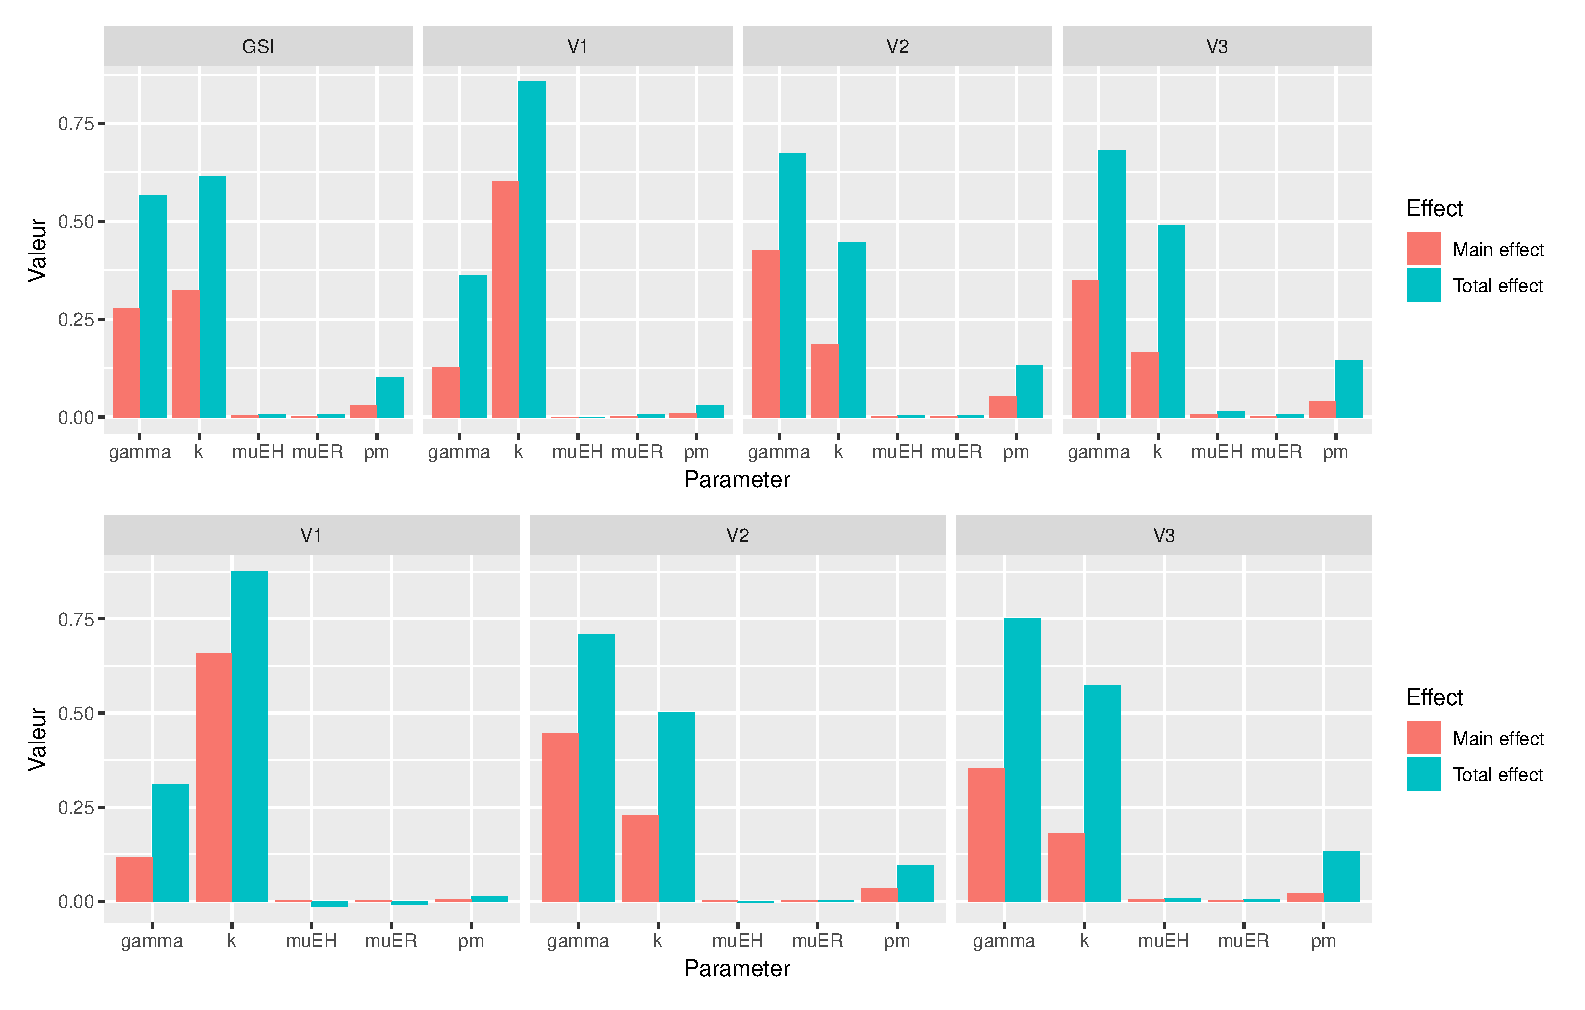
\epsfig{file=sa.eps, width = 10.8cm}
 % larves_grid_nolegend.pdf: 655x392 px, 72dpi, 23.11x13.83 cm, bb=0 0 655 392
 \caption{Analyses de sensibilité : méthodes Dynamic Sensitivity Indices (en haut) et Sobol (en bas)}
\end{figure}
\end{frame}

\begin{frame}
 \begin{figure}
 \centering
 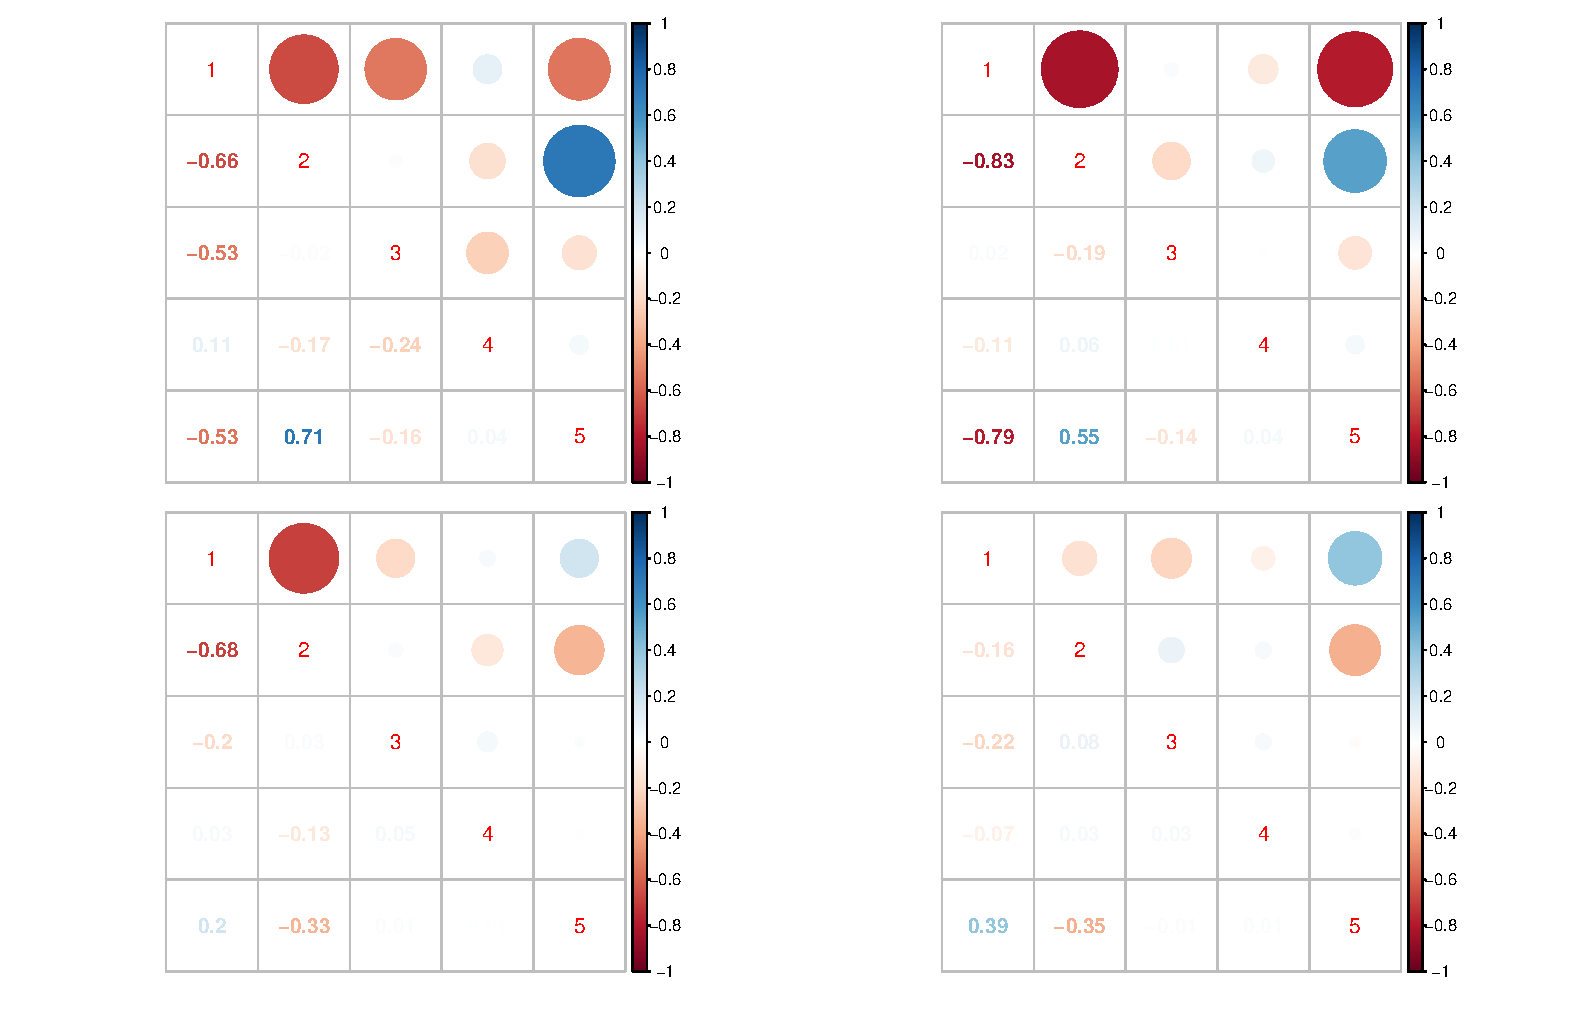
\epsfig{file=matcor.eps, width = 10.8cm}
 % larves_grid_nolegend.pdf: 655x392 px, 72dpi, 23.11x13.83 cm, bb=0 0 655 392
 \caption{Matrices de correlations des paramètres renvoyés par Differential Evolution et NSGA--II ($\min \|\cdot\|_1, \min \|\cdot\|_2, \min \|\cdot\|_\infty$)}
\end{figure}
\end{frame}

\begin{frame}
  \begin{figure}
 \centering
 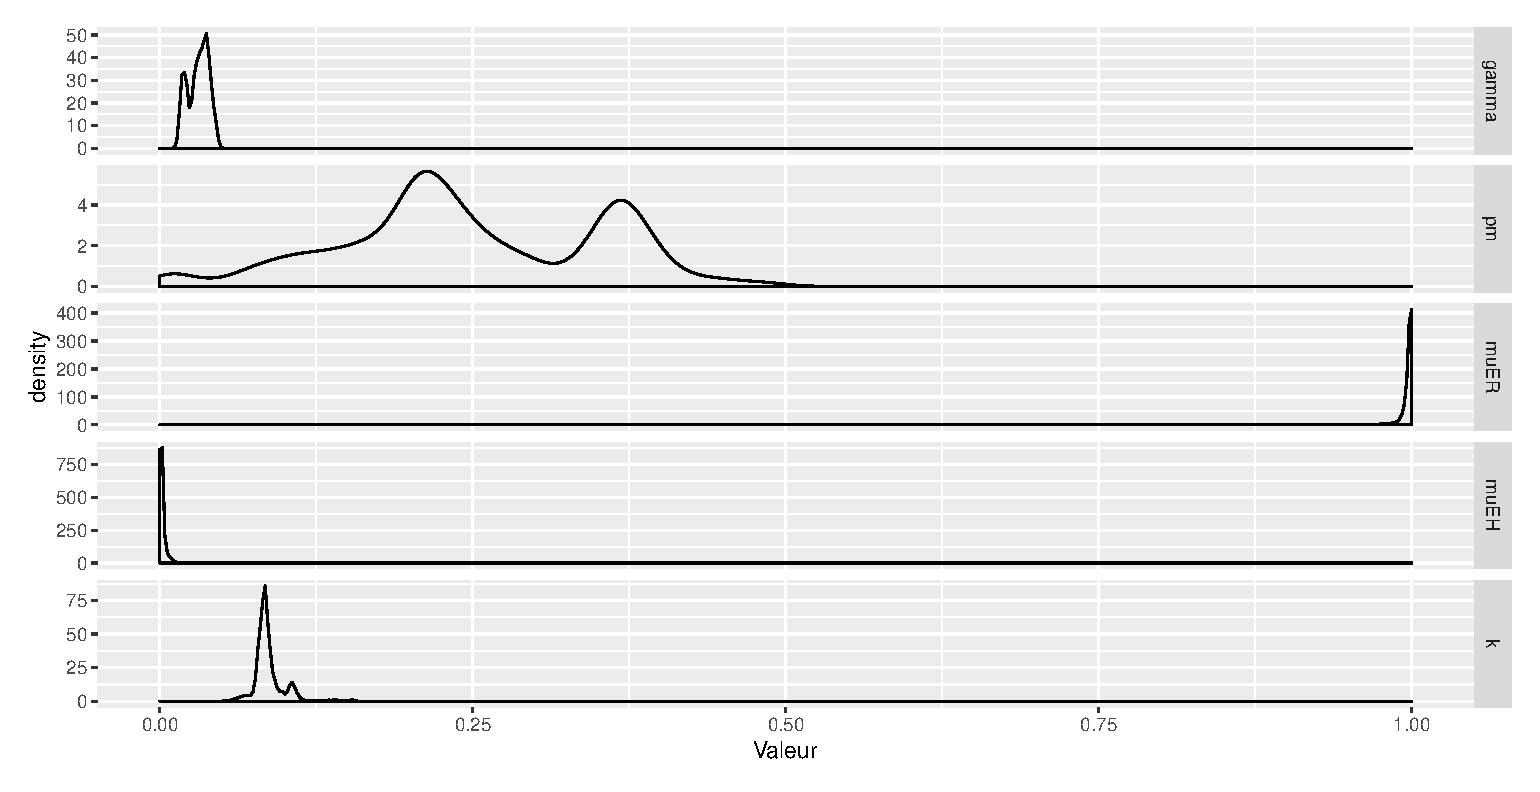
\epsfig{file=densities.eps, width = 10.8cm}
 % larves_grid_nolegend.pdf: 655x392 px, 72dpi, 23.11x13.83 cm, bb=0 0 655 392
 \caption{Densités des différents paramètres obtenus par l'algo NSGA-II}
\end{figure}
\end{frame}

\begin{frame}
  \begin{figure}
 \centering
 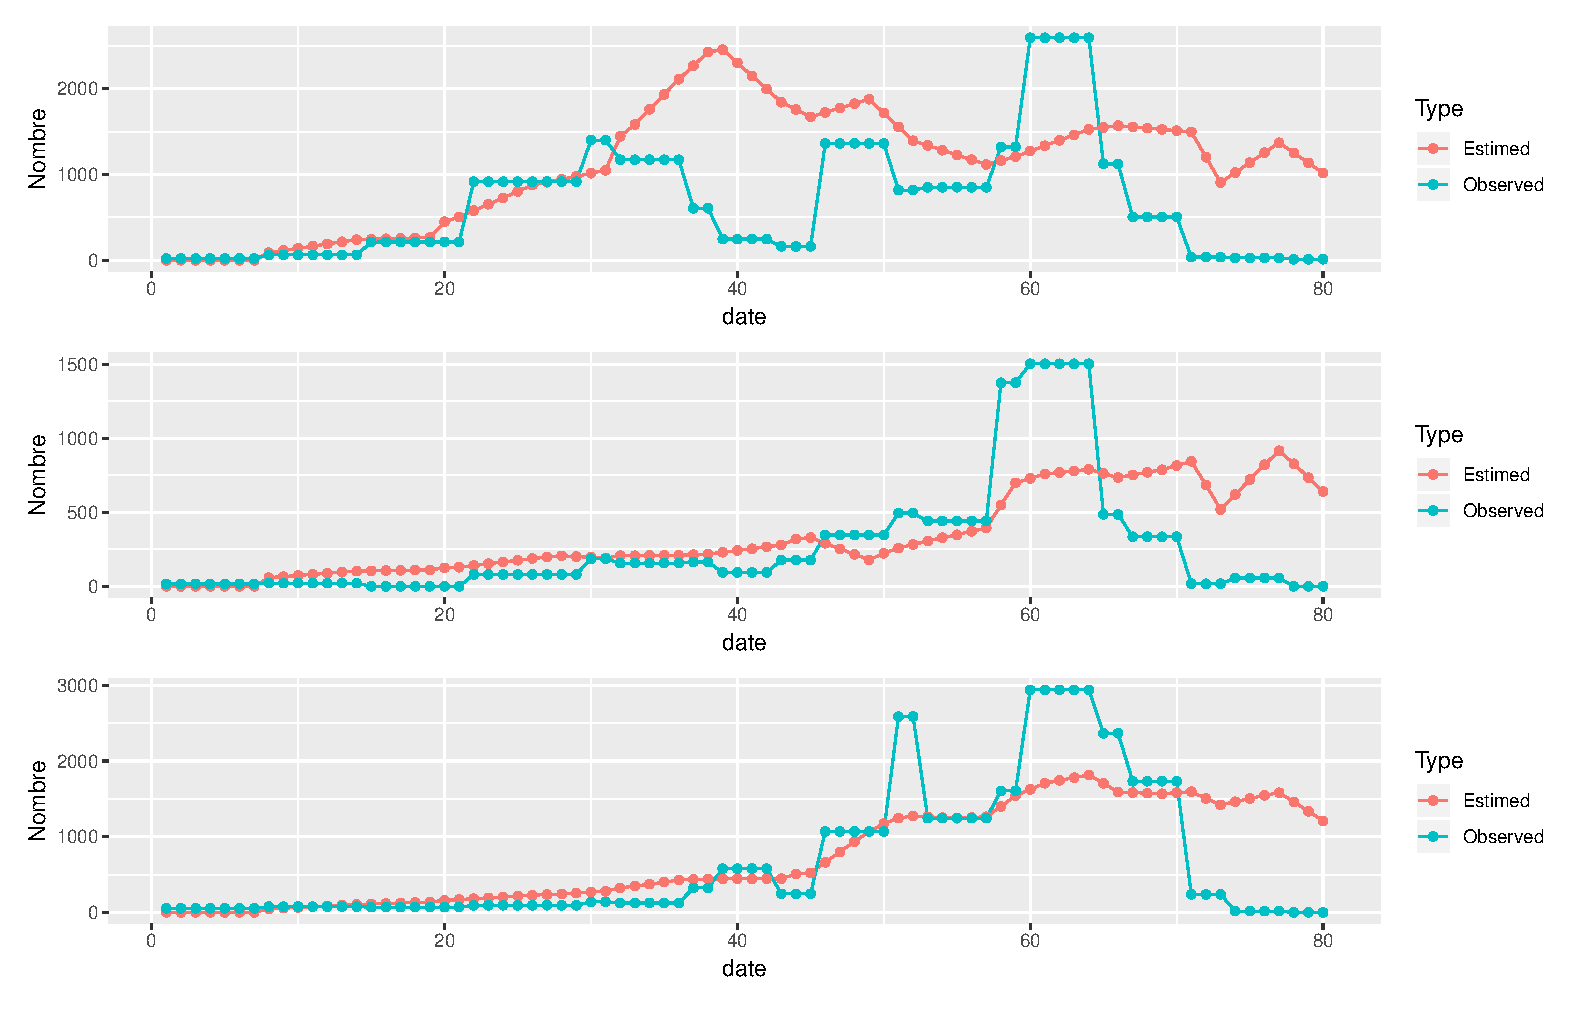
\epsfig{file=last.eps, scale = 0.4}
 % larves_grid_nolegend.pdf: 655x392 px, 72dpi, 23.11x13.83 cm, bb=0 0 655 392
 \caption{Simulation du nombre de larves après avoir fixé $\mu_{ER}$ et $\mu_{EH}$ en utilisant les paramètres obtenus grâce à NSGA-II ($\min \|\cdot\|_2$)}
\end{figure}
\end{frame}

\begin{frame}
 Perspectives d'améliorations :
 \begin{itemize}
 \item prendre en compte les individus en diapause ;
 \item températures ;
 \item prendre en compte le stade phénologiques des inflorescences.
 \end{itemize}

\end{frame}





 
\end{document}

